\section{Problemi considerati}
\subsection{Alcune definizioni fondamentali}
Per definire formalmente il concetto di grafo è necessario introdurre la definizione di relazione binaria.
\begin{definition}
    Chiameremo relazione binaria su $A,B$ qualsiasi sottoinsieme del prodotto cartesiano $A \times B$.\\
    Chiameremo relazione binaria su $A$ qualsiasi sottoinsieme del prodotto cartesiano $A \times A$.\\
    Diremo che $u,v$ sono in relazione rispetto a $b$ se $(u,v) \in b$. In questo caso useremo la notazione $u \,b\, v$.
\end{definition}
\begin{definition}
    Sia $b$ una relazione binaria su $N$.
    Diamo le seguenti definizioni
    \begin{itemize}
        \item Chiusura riflessiva: $b_r = b \cup \{(x,x) \,\, \forall x \in N\}$
        \item Chiusura simmetrica: $b_s = b \cup \{(y,x) \,\, \forall x,y : (x,y) \in b\}$
        \item Chiusura transitiva: $b_t = b \cup \{(x,z) \,\, \forall x,z : \exists y : (x,y) \in b \land (y,z) \in b\}$
    \end{itemize}
\end{definition}
\begin{definition}
    Sia $N \neq \emptyset$. Sia $\to$ una relazione binaria su $N$.\\
    Chiameremo grafo la coppia $G = (N, \to)$.\\
    In questo caso
    \begin{itemize}
        \item $N$ è l'insieme dei nodi;
        \item $\to$ è la relazione di raggiungibilità: $a \to b \,\,(a,b \in N)$ significa "nel grafo $G$ esiste un arco dal nodo $a$ al nodo $b$".
    \end{itemize}
\end{definition}
\begin{example}
    \begin{figure}[b]
        \centering
        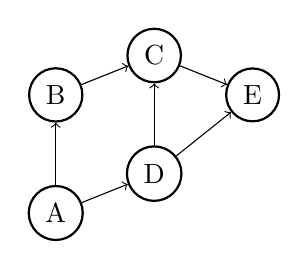
\begin{tikzpicture}[scale=0.5]
            \begin{scope}[every node/.style={circle,thick,draw}]
                \node (A) at (0,0) {A};
                \node (B) at (0,3) {B};
                \node (C) at (2.5,4) {C};
                \node (D) at (2.5,1) {D};
                \node (E) at (5,3) {E} ;
            \end{scope}

            \begin{scope}
                \path [->] (A) edge node {} (B);
                \path [->] (B) edge node {} (C);
                \path [->] (A) edge node {} (D);
                \path [->] (D) edge node {} (C);
                \path [->] (D) edge node {} (E);
                \path [->] (C) edge node {} (E);
            \end{scope}
            \end{tikzpicture}
        \caption{}
    \end{figure}
    Il grafo di Figura 1 è descritto dalla coppia
    \begin{itemize}
        \item $N = \{A,B,C,D,E\}$
        \item $\to \,\,= \{(A,B), (A,D), (B,C), (D,C), (C,E), (D,E)\}$
    \end{itemize}
\end{example}
\subsection{Bisimulazione}
\begin{definition}
    Siano $G_1 = (N_1, E_1), G_2 = (N_2, E_2)$ due grafi. Diremo che $G_1, G_2$ sono bisimili \cite{dovier} rispetto alla relazione binaria $b$ su $N_1, N_2$ se $\forall u \in N_1, v \in N_2$ valgono congiuntamente le seguenti condizioni
    \begin{itemize}
        \item $\forall u' \in N_1 : u \to u', u \,b\, v \implies \,\exists v' \in N_2 : (u' \,b\, v' \land v \to v')$
        \item $\forall v' \in N_2 : v \to v', u \,b\, v \implies \,\exists u' \in N_1 : (u' \,b\, v' \land u \to u')$
    \end{itemize}
\end{definition}
Per introdurre risultati che verranno presentati in seguito risulta utile definire la bisimulazione su un grafo:
\begin{definition}
    Sia $G = (N, \to)$ un grafo, e $b$ una relazione binaria su $N$. Diremo che $b$ è una bisimulazione su $G$ se $\forall u,v \in N$ valgono congiuntamente le seguenti condizioni
    \begin{itemize}
        \item $\forall u' \in N : u \to u', u \,b\, v \implies \,\exists v' \in N : (u' \,b\, v' \land v \to v')$
        \item $\forall v' \in N : v \to v', u \,b\, v \implies \,\exists u' \in N : (u' \,b\, v' \land u \to u')$
    \end{itemize}
\end{definition}
\begin{proposition}
    Sia $b$ una bisimulazione sul grafo $G$. La sua chiusura riflessiva, simmetrica o transitiva è ancora una bisimulazione su $G$.
\end{proposition}
\begin{proof}[Dimostrazione] Considero separatamente le tre relazioni $b_r, b_s, b_t$, rispettivamente la chiusura riflessiva, simmetrica e transitiva:
    \begin{itemize}
        \item[$b_r$] Per definizione $b \subset b_r$, quindi è sufficiente dimostrare che $b_r$ è una bisimulazione solo quando gli argomenti $u,v \in N$ non sono distinti.\\
        Sia $u \in N$. Chiaramente $u \,b_r\, u$. Se $\exists u' \in N : u \to u' \implies u' \,b_r\, u'$.
        \item[$b_s$] Per definizione $b \subset b_s$, quindi è sufficiente dimostrare che $b_s$ è una bisimulazione quando per gli argomenti $u,v \in N$ si ha $u \,b\, v$ ma non $v \,b\, u$.\\
        Sia $(u,v) \in N \times N$ una coppia con questa proprietà. Allora vale $u \,b\, v \land v \,b_s\, u$. Per la prima relazione si deduce che se $\exists v' \in N : v \to v' \implies \exists u' \in N : (u \to u' \land u' \,b\,v')$. Allora $v' \,b_s\, u'$. In modo speculare si dimostra la seconda parte della proprietà caratteristica della bisimulazione.
        \item[$b_t$] Per definizione $b \subset b_t$, quindi è sufficiente dimostrare che $b_t$ è una bisimulazione quando per gli argomenti $u,v,z \in N$ si ha $u \,b\, v$, $v \,b\, z$ ma non $u \,b\, z$.\\
        Sia $(u,v,z) \in N \times N \times N$ con questa proprietà. Allora se $\exists u', v' \in N : u \to u' \implies \exists v' \in N : v \to v' \land u' \,b\, v'$. Inoltre $\exists z' : z \to z' \land v' \,b\, z'$.\\
        Ricapitolando si ha $u' \,b\, v', v' \,b\, z'$. Allora per definizione di $b_t: u' \,b_t\, z'$. In modo speculare si ottiene la seconda parte della proprietà caratteristica della bisimulazione.
    \end{itemize}
\end{proof}
\begin{corollary}
    Ad ogni bisimulazione $b$ si può associare una bisimulazione $\widetilde{b} : b \subset \widetilde{b} \,\,\land\,\, \widetilde{b}$ è una relazione di equivalenza.
\end{corollary}
